%
% ISoLA 2020
%
% http://isola-conference.org/isola2020/
%
% 31 May 2020     Paper Submission
% 29 June 2020    Reports and Notification
% 02 August 2020  Final Versions
%
% Conference: Rhodes, October 26th - October 30th 2020
%
% "The expected length is around 15 pages with some flexibility in case of need."
%

% There doesn't appear to be any anonymity requirement

\documentclass[runningheads]{llncs}
\usepackage{lineno}
%\linenumbers

% correct bad hyphenation here
\hyphenation{}

%\usepackage{natbib}
\usepackage{url}

% *** MATHS PACKAGES ***
%
\usepackage[cmex10]{amsmath}
\usepackage{amssymb}
\usepackage{stmaryrd}
%% \usepackage{amsthm}
\usepackage{proof}


% *** ALIGNMENT PACKAGES ***
%
\usepackage{array}
\usepackage{float}  %% Try to improve placement of figures.  Doesn't work well with subcaption package.
\usepackage{subcaption}
\usepackage{caption}

\usepackage{geometry}
\usepackage{listings}
\usepackage[dvipsnames]{xcolor}
\usepackage{verbatim}
\usepackage{alltt}
\usepackage{paralist}

\usepackage{todonotes}
%\usepackage[disable]{todonotes}

% This has to go at the end of the packages.
\usepackage[colorlinks=true,linkcolor=MidnightBlue,citecolor=ForestGreen,urlcolor=Plum]{hyperref}

\newcommand\ifootnote[1]{(#1)}
%% ^ inline footnote

\newcommand\site[1]{\footnote{\url{#1}}}
%% ^ footnote URL

% Tikz
\usepackage{tikz}
\usetikzlibrary{arrows,positioning,matrix,fit,decorations.text}

% Stuff for splitting figures over page breaks
%\DeclareCaptionLabelFormat{continued}{#1~#2 (Continued)}
%\captionsetup[ContinuedFloat]{labelformat=continued}

% *** MACROS ***

\newcommand{\todochak}[1]{\todo[inline,color=purple!40,author=chak]{#1}}
\newcommand{\todompj}[1]{\todo[inline,color=yellow!40,author=Michael]{#1}}
\newcommand{\todokwxm}[1]{\todo[inline,color=blue!20,author=kwxm]{#1}}
\newcommand{\todojm}[1]{\todo[inline,color=purple!40,author=Jann]{#1}}
\newcommand{\todor}[1]{\todo[inline,color=red!40,author=Orestis]{#1}}
\newcommand{\todojmc}[1]{\todo[inline,color=green!40,author=James]{#1}}

\newcommand{\red}[1]{\textcolor{red}{#1}}
\newcommand{\redfootnote}[1]{\red{\footnote{\red{#1}}}}
\newcommand{\blue}[1]{\textcolor{blue}{#1}}
\newcommand{\bluefootnote}[1]{\blue{\footnote{\blue{#1}}}}

%% A version of ^{\prime} for use in text mode
\makeatletter
\DeclareTextCommand{\textprime}{\encodingdefault}{%
  \mbox{$\m@th'\kern-\scriptspace$}%
}
\makeatother

\renewcommand{\i}{\textit}  % Just to speed up typing: replace these in the final version
\renewcommand{\t}{\texttt}  % Just to speed up typing: replace these in the final version
\newcommand{\s}{\textsf}  % Just to speed up typing: replace these in the final version
\newcommand{\msf}[1]{\ensuremath{\mathsf{#1}}}
\newcommand{\mi}[1]{\ensuremath{\mathit{#1}}}

%% A figure with rules above and below.
\newcommand\rfskip{7pt}
%\newenvironment{ruledfigure}[1]{\begin{figure}[#1]\hrule\vspace{\rfskip}}{\vspace{\rfskip}\hrule\end{figure}}
\newenvironment{ruledfigure}[1]{\begin{figure}[#1]}{\end{figure}}

%% Various text macros
\newcommand{\true}{\ensuremath{\mathsf{true}}} % \textsf becomes slanted in math mode
\newcommand{\false}{\ensuremath{\textsf{false}}}

\newcommand{\hash}[1]{\ensuremath{#1^{\#}}}

\newcommand{\List}[1]{\ensuremath{\s{List}[#1]}}
\newcommand{\Set}[1]{\ensuremath{\s{Set}[#1]}}
\newcommand{\FinSet}[1]{\ensuremath{\s{FinSet}[#1]}}
\newcommand{\Interval}[1]{\ensuremath{\s{Interval}[#1]}}
\newcommand{\FinSup}[2]{\ensuremath{\s{FinSup}[#1,\linebreak[0]#2]}}
% ^ \linebreak is to avoid a bad line break when we talk about finite
% maps.  We may be able to remove it in the final version.

\newcommand{\supp}{\msf{supp}}

\newcommand{\Script}{\ensuremath{\s{Script}}}
\newcommand{\scriptAddr}{\msf{scriptAddr}}
\newcommand{\ctx}{\ensuremath{\s{Context}}}
\newcommand{\vlctx}{\ensuremath{\s{ValidatorContext}}}
\newcommand{\mpsctx}{\ensuremath{\s{PolicyContext}}}
\newcommand{\toData}{\ensuremath{\s{toData}}}
\newcommand{\toTxData}{\ensuremath{\s{toTxData}}}
\newcommand{\fromData}{\msf{fromData}}

\newcommand{\mkContext}{\ensuremath{\s{mkContext}}}
\newcommand{\mkVlContext}{\ensuremath{\s{mkValidatorContext}}}
\newcommand{\mkMpsContext}{\ensuremath{\s{mkPolicyContext}}}

\newcommand{\applyScript}[1]{\ensuremath{\llbracket#1\rrbracket}}
\newcommand{\applyMPScript}[1]{\ensuremath{\llbracket#1\rrbracket}}

% Macros for eutxo things.
\newcommand{\tx}{\mi{tx}}
\newcommand{\TxId}{\ensuremath{\s{TxId}}}
\newcommand{\txId}{\msf{txId}}
\newcommand{\txrefid}{\mi{id}}
\newcommand{\Address}{\ensuremath{\s{Address}}}
\newcommand{\DataHash}{\ensuremath{\s{DataHash}}}
\newcommand{\hashData}{\msf{dataHash}}
\newcommand{\idx}{\mi{index}}
\newcommand{\inputs}{\mi{inputs}}
\newcommand{\outputs}{\mi{outputs}}
\newcommand{\forge}{\mi{forge}}
\newcommand{\forgeScripts}{\mi{forgeScripts}}
\newcommand{\sigs}{\mi{sigs}}
\newcommand{\fee}{\mi{fee}}
\newcommand{\addr}{\mi{addr}}
\newcommand{\val}{\mi{value}}  %% \value is already defined

\newcommand{\validator}{\mi{validator}}
\newcommand{\redeemer}{\mi{redeemer}}
\newcommand{\datum}{\mi{datum}}
\newcommand{\datumHash}{\mi{datumHash}}
\newcommand{\datumWits}{\mi{datumWitnesses}}
\newcommand{\Data}{\ensuremath{\s{Data}}}
\newcommand{\Input}{\ensuremath{\s{Input}}}
\newcommand{\Output}{\ensuremath{\s{Output}}}
\newcommand{\OutputRef}{\ensuremath{\s{OutputRef}}}
\newcommand{\Signature}{\ensuremath{\s{Signature}}}
\newcommand{\Ledger}{\ensuremath{\s{Ledger}}}

\newcommand{\outputref}{\mi{outputRef}}
\newcommand{\outputrefs}{\mi{outputRefs}}
\newcommand{\txin}{\mi{in}}
\newcommand{\id}{\mi{id}}
\newcommand{\lookupTx}{\msf{lookupTx}}
\newcommand{\getSpent}{\msf{getSpentOutput}}

\newcommand{\Tick}{\ensuremath{\s{Tick}}}
\newcommand{\currentTick}{\msf{currentTick}}
\newcommand{\spent}{\msf{spentOutputs}}
\newcommand{\unspent}{\msf{unspentOutputs}}
\newcommand{\txunspent}{\msf{unspentTxOutputs}}
\newcommand{\eutxotx}{\msf{Tx}}

\newcommand{\Quantity}{\ensuremath{\s{Quantity}}}
\newcommand{\Asset}{\ensuremath{\s{Asset}}}
\newcommand{\Policy}{\ensuremath{\s{Policy}}}
\newcommand{\Quantities}{\ensuremath{\s{Quantities}}}
\newcommand{\nativeCur}{\ensuremath{\mathrm{nativeC}}}
\newcommand{\nativeTok}{\ensuremath{\mathrm{nativeT}}}

\newcommand\B{\ensuremath{\mathbb{B}}}
\newcommand\N{\ensuremath{\mathbb{N}}}
\newcommand\Z{\ensuremath{\mathbb{Z}}}
\renewcommand\H{\ensuremath{\mathbb{H}}}
%% \H is usually the Hungarian double acute accent
\newcommand{\emptyBs}{\ensuremath{\emptyset}}

\newcommand{\emptymap}{\ensuremath{\{\}}}

\newcommand{\outRef}{\mi{out}_{\mi{ref}}}
\newcommand{\fps}{\mi{fps}}
\newcommand{\fpss}{\mi{fpss}}

\usepackage{etoolbox}

\newcommand{\Bcc}{Bcc}
\newcommand{\ZerepochCore}{Zerepoch Core}
\newcommand{\GitUser}{omelkonian}

% Macros for formalisation
\newcommand\agdaRepo{https://github.com/omelkonian/formal-utxo/tree/2d32}
\newcommand\ra{\rightarrow}
\newcommand\nft{\blacklozenge}
\newcommand\NF{\s{NonFungible}}
\newcommand\Trace{\s{Trace}}
\newcommand\Provenance{\s{Provenance}}
\newcommand\provenance{\s{provenance}}
\newcommand\isFinal{\msf{isFinal}}
\newcommand\step{\msf{step}}
\newcommand\satisfies{\msf{satisfies}}
\newcommand\checkOutputs{\msf{checkOutputs}}
\newcommand\initial{\msf{initial}}
\newcommand\extract{\msf{extract}}

\newcommand\All{\msf{All}}
\newcommand\AllS{\msf{All}^\s{S}}

\newcommand\mkValidator[1]{\msf{validator}_#1}
\newcommand\mkPolicy[1]{\msf{policy}_#1}
\newcommand\valC{\mkValidator{\mathcal{C}}}
\newcommand\polC{\mkPolicy{\mathcal{C}}}

\newcommand\CStepArrow[3]{\ensuremath{
#1 \xrightarrow{\hspace{5pt} #2 \hspace{5pt}} (#1' , #3)
}}

\newcommand\txeq{tx^\equiv}
\newcommand\Sim[2]{\ensuremath{
#1 \sim #2
}}
\newcommand\CStep[1]{\ensuremath{
 #1 \xrightarrow{\hspace{5pt} i \hspace{5pt}} (#1' , \txeq)
%%\textsf{step}\, #1\, i \equiv \textsf{just}\, #1'
}}
\newcommand\LStep[2]{\ensuremath{
#1 \xrightarrow{\hspace{5pt} #2 \hspace{5pt}} #1'
}}
\newcommand\transTo{\ensuremath{
    \rightsquigarrow^*
}}
\newcommand\transToN{\ensuremath{
    \rightsquigarrow^{+}
}}

% multisig
\newcommand{\msc}{\mathrm{msc}}
\newcommand{\sig}{\mathit{sig}}
%\newcommand{\sigs}{\mathit{sigs}}
\newcommand{\auth}{\mathrm{auth}}
\newcommand{\Holding}{\msf{Holding}}
\newcommand{\Collecting}[4]{\msf{Collecting}(#1, #2, #3, #4)}
\newcommand{\Propose}[3]{\msf{Propose}(#1, #2, #3)}
\newcommand{\Add}[1]{\msf{Add}(#1)}
\newcommand{\Cancel}{\msf{Cancel}}
\newcommand{\Pay}{\msf{Pay}}

% Names, for consistency
\newcommand{\UTXO}{UTXO}
\newcommand{\EUTXO}{E\UTXO{}}
\newcommand{\ExUTXO}{Extended \UTXO{}}
\newcommand{\CEM}{CEM}
\newcommand{\UTXOma}{\UTXO$_{\textrm{ma}}$}
\newcommand{\EUTXOma}{\EUTXO$_{\textrm{ma}}$}

\newcommand{\diffBox}[1]{\text{\colorbox{lightgray}{\(#1\)}}}

% relaxed float placement
\renewcommand{\topfraction}{.95}
\renewcommand{\bottomfraction}{.7}
\renewcommand{\textfraction}{.15}
\renewcommand{\floatpagefraction}{.66}
\renewcommand{\dbltopfraction}{.66}
\renewcommand{\dblfloatpagefraction}{.66}
\setcounter{topnumber}{9}
\setcounter{bottomnumber}{9}
\setcounter{totalnumber}{20}
\setcounter{dbltopnumber}{9}

%% ------------- Start of document ------------- %%

\begin{document}

\title{Native Custom Tokens in the Extended \UTXO{} Model}

% First names are abbreviated in the running head.
% If there are more than two authors, 'et al.' is used.

\author{
  Manuel M.T. Chakravarty\inst{1}
  \and
  James Chapman\inst{1}
  \and
  Kenneth MacKenzie\inst{1}
  \and
  Orestis Melkonian\inst{1,2}
  \and
  Jann M\"uller\inst{1}
  \and
  Michael Peyton Jones\inst{1}
  \and
  Polina Vinogradova\inst{1}
  \and
  Philip Wadler\inst{1,2}
}

\authorrunning{Chakravarty et al.}

\institute{
  The Blockchain Co.,
  \email{firstname.lastname@bcccoin.io}
  \and
  University of Edinburgh,
  \email{orestis.melkonian@ed.ac.uk, wadler@inf.ed.ac.uk}
}

\maketitle

\begin{abstract}
  \emph{User-defined tokens} ---both fungible ERC-20 and non-fungible ERC-721 tokens--- are central to the majority of contracts deployed on Ethereum. User-defined tokens are \emph{non-native} on Ethereum; i.e., they are not directly supported by the ledger, but require custom code. This makes them unnecessarily inefficient, expensive, and complex.

  The \emph{Extended UTXO Model} (\kern-0.5pt\emph{\EUTXO})~\cite{eutxo-1-paper} has been introduced as a generalisation of Bitcoin-style \UTXO\ ledgers, allowing support of more expressive smart contracts, approaching the functionality available to contracts on Ethereum. Specifically, a bisimulation argument established a formal relationship between the \EUTXO\ ledger and a general form of state machines. Nevertheless, \emph{transaction outputs} in the \EUTXO\ model lock integral quantities of a single native cryptocurrency only, just like Bitcoin.

  In this paper, we study a generalisation of the \EUTXO\ ledger model with \emph{native} user-defined tokens. Following the approach proposed in a companion paper~\cite{plain-multicurrency} for the simpler case of plain Bitcoin-style \UTXO\ ledgers, we generalise transaction outputs to lock not merely coins of a single cryptocurrency, but entire \emph{token bundles,} including custom tokens whose forging is controlled by \emph{forging policy scripts.} We show that this leads to a rich ledger model that supports a broad range of interesting use cases.

  Our main technical contribution is a formalisation of the multi-asset \EUTXO\ ledger in Agda, which we use to establish that the ledger with custom tokens is strictly more expressive than the original \EUTXO\ ledger. In particular, we state and prove a transfer result for inductive and temporal properties from state machines to the multi-asset \EUTXO\ ledger, which was out of scope for the single-currency \EUTXO\ ledger. In practical terms, the resulting system is the basis for the smart contract system of the Bcc blockchain.
\end{abstract}

\keywords{blockchain \and \UTXO{} \and tokens \and functional
  programming \and state machines \and bisimulation}

\section{Introduction}

If we look at contracts on Ethereum in terms of their use and the monetary values that they process, then it becomes apparent that so-called \emph{user-defined} (or \emph{custom}) \emph{tokens} play a central role in that ecosystem. The two most common token types are \emph{fungible tokens}, following the ERC-20 standard~\cite{ERC-20}, and \emph{non-fungible} tokens, following the ERC-721 standard~\cite{ERC-721}.
% This footnote is IMHO superflous. The dictionary definition of "fungible" is " replaceable by another identical item; mutually interchangeable", which seems to perfectly fit with our use and we use the term as it is usually used in the context of cryptocurrencies. (This footnote also screws up the frontpage.)
%\footnote{
%  Fungibility is strictly a relation between objects, rather than a property of a single object. However, throughout this paper we will follow the common pattern of describing an object as (non-)fungible when it is (non-)fungible with all other objects in some appropriate reference class, which should be clear from context (e.g. a ``fungible token'' is fungible with all the other tokens in its asset group, but not outside that). We may also refer to a set of objects as (non-)fungible when they are all (non-)fungible with each other.
%}

On Ethereum, ERC-20 and ERC-721 tokens are fundamentally different from the native cryptocurrency, Ether, in that their creation and use always involves user-defined custom code --- they are not directly supported by the underlying ledger, and hence are \emph{non-native}.  This makes them unnecessarily inefficient, expensive, and complex. Although the ledger already includes facilities to manage and maintain a currency, this functionality is replicated in interpreted user-level code, which is inherently less efficient. Moreover, the execution of user-code needs to be paid for (in gas), which leads to significant costs. Finally, the ERC-20 and ERC-721 token code gets replicated and adapted, instead of being part of the system, which complicates the creation and use of tokens and leaves room for human error.

The alternative to user-level token code is a ledger that supports \emph{native tokens}. In other words, a ledger that directly supports
\begin{inparaenum}[(1)]
\item the creation of new user-defined token or asset types,
\item the forging of those tokens, and
\item the transfer of custom token ownership between multiple participants.
\end{inparaenum}
In a companion paper~\cite{plain-multicurrency}, we propose a generalisation of Bitcoin-style \UTXO\ ledgers, which we call \UTXOma (``ma'' for ``multi-asset''), adding native tokens by way of so-called \emph{token bundles} and domain-specific \emph{forging policy scripts}, without the need for a general-purpose scripting system.

Independently, we previously introduced the \emph{Extended UTXO Model} (\EUTXO)~\cite{eutxo-1-paper} as an orthogonal generalisation of Bitcoin-style \UTXO\ ledgers, enabling support of more expressive smart contracts, with functionality similar to contracts on Ethereum. To support user-defined tokens or currencies on \EUTXO, we could follow Ethereum's path and define standards corresponding to ERC-20 and ERC-721 for fungible and non-fungible tokens, but then we would be subject to the same disadvantages that non-native tokens have on Ethereum.

In this paper, to avoid the disadvantages of non-native tokens, we investigate the combination of the two previously mentioned extensions of the plain \UTXO\ model: we add \UTXOma-style token bundles and asset policy scripts to the \EUTXO\ model, resulting in a new \EUTXOma\ ledger model.

We will show that the resulting \EUTXOma\ model is strictly more expressive than both \EUTXO\ and \UTXOma\ by itself. In particular, the constraint-emitting state machines in~\cite{eutxo-1-paper} can not ensure that they are initialised correctly. In \EUTXOma, we are able to use non-fungible tokens to trace \emph{threads} of state machines. Extending the mechanised Agda model from~\cite{eutxo-1-paper} allows us to then prove inductive and temporal properties of state machines by induction over their traces, covering a wide variety of state machine correctness properties.

Moreover, the more expressive scripting functionality and state threading of \EUTXO\ enables us to define more sophisticated asset policies than in \UTXOma. Additionally, we argue that the combined system allows for sophisticated access-control schemes by representing roles and capabilities in the form of user-defined tokens.

In summary, this paper makes the following contributions:
%
\begin{itemize}
\item We introduce the multi-asset \EUTXOma\ ledger model (\S\ref{sec:EUTXOma}).
\item We outline a range of application scenarios that are arguably better supported by the new model, and also applications that plain \UTXOma\ does not support at all (\S\ref{sec:applications}).
\item We formally prove a transfer result for inductive and temporal properties from constraint emitting machines to the \EUTXOma\ ledger, an important property that we were not able to establish for plain \EUTXO\ (\S\ref{sec:formalization}).
\end{itemize}
%
We discuss related work in \S\ref{sec:related-work}. Due to space constraints, the formal ledger rules for \EUTXOma\ are in Appendix~\ref{app:model}. A mechanised version of the ledger rules and the various formal results from \S\ref{sec:formalization} is available as Agda source code.\footnote{\url{\agdaRepo}}

On top of the conceptual and theoretical contributions made in this paper, we would like to emphasise that the proposed system is highly practical. In fact, \EUTXOma\ underlies our implementation of \emph{Zerepoch Platform,} the smart contract system of the Bcc blockchain.\footnote{\url{https://github.com/The-Blockchain-Company/zerepoch}}

\section{Extending Extended \UTXO}
\label{sec:EUTXOma}

Before discussing applications and the formal model of \EUTXOma, we briefly summarise the structure of \EUTXO, and then informally introduce the multi-asset extension that is the subject of this paper.
Finally, we will discuss a shortcoming in the state machine mapping of \EUTXO\ as introduced in~\cite{eutxo-1-paper} and illustrate how the multi-asset extension fixes that shortcoming.

\subsection{The starting point: Extended \UTXO}
\label{sec:informal-eutxo}

In Bitcoin's \UTXO\ ledger model, the ledger is formed by a list of transactions grouped into blocks.
As the block structure is secondary to the discussion in this paper, we will disregard it in the following.
A transaction $\tx$ is a quadruple \((I, O, r, S)\) comprising a set of \emph{inputs} $I$, a list of \emph{outputs} $O$, a \emph{validity interval} $r$, and a set of signatures $S$, where inputs and outputs represent cryptocurrency value flowing into and out of the transaction, respectively.
The sum of the inputs must be equal to the sum of the outputs; in other words, transactions preserve value.
% True, but not crucial IMHO and we need to save space. -= chak
%\footnote{
%  Real transactions will likely have other fields that need to be balanced, such as fees or new tokens that are minted or forged.
%  We will omit these for now for simplicity, but in general they also need to observe preservation of value.
%}
Transactions are identified by a collision-resistant cryptographic hash $h$ computed from the transaction.\footnote{%
  We denote the hash of some data $d$ as $d^\#$.%
}

An input $i\in I$ is represented as a pair \((\outRef, \rho)\) of an \emph{output reference} $\outRef$ and a \emph{redeemer value} $\rho$.
The output reference $\outRef$ uniquely identifies an output in a preceding transaction by way of the transaction's hash and the output's position in the transaction's list of outputs.

In plain \UTXO, an output $o\in O$ is a pair of a \emph{validator script} $\nu$ and cryptocurrency value $\val$.
In the Extended \UTXO\ model (\EUTXO)~\cite{eutxo-1-paper}, outputs become triples \((\nu, \val, \delta)\), where the added \emph{datum} $\delta$ enables passing additional information to the validator.

The purpose of the validator is to assess whether an input $i$ of a subsequent transaction trying to spend (i.e., consume) an output $o$ should be allowed to do so.
To this end, we execute the validator script to check whether \(\nu(\rho, \delta, \sigma) = \true\) holds.
Here $\sigma$ comprises additional information about the \emph{validation context} of the transaction.
In the plain \UTXO\ model that contextual information is fairly limited: it mainly consists of the validated transaction's hash, the signatures $S$, and information about the length of the blockchain. In the \EUTXO\ model, we extend $\sigma$ to include the entirety of the validated transaction $\tx$ as well as all the outputs spent by the inputs of $\tx$.

\subsection{Token bundles}
\label{sec:informal-token-bundles}

In \UTXO\ and \EUTXO, the $\val$ carried by an output is represented as an integral value denoting a specific quantity of the ledger's native cryptocurrency.
As discussed in more detail in the companion paper~\cite{plain-multicurrency}, we can generalise $\val$ to carry a two-level structure of \emph{finitely-supported functions.}
The technicalities are in Appendix~\ref{app:model}; for now, we can regard them as nested finite maps to quantities of tokens.
For example, the value
\(\{\mathsf{Coin} \mapsto \{\mathsf{Coin} \mapsto 3\}, g \mapsto \{t_1
\mapsto 1, t_2 \mapsto 1\}\}\) contains $3$ $\mathsf{Coin}$ coins
(there is only one (fungible) token $\mathsf{Coin}$ for a payment
currency also called $\mathsf{Coin}$), as well as (non-fungible) tokens $t_1$ and $t_2$,
both in asset group $g$.  Values can be added naturally, e.g.,
\begin{align*}
 & \{\mathsf{Coin} \mapsto \{\mathsf{Coin} \mapsto 3\}, g \mapsto \{t_1
   \mapsto 1, t_2 \mapsto 1\}\} \\
 + \ & \{\mathsf{Coin} \mapsto \{\mathsf{Coin} \mapsto 1\}, g \mapsto \{t_3 \mapsto 1\}\} \\
 = \ & \{\mathsf{Coin} \mapsto \{\mathsf{Coin} \mapsto 4\}, g \mapsto \{t_1
       \mapsto 1, t_2 \mapsto 1, t_3 \mapsto 1\}\} \ .
\end{align*}
%
In a bundle, such as \(g \mapsto \{t_1 \mapsto 1, t_2 \mapsto 1, t_3 \mapsto 1\}\), we call $g$ an \emph{asset group} comprising a set of tokens $t_1$, $t_2$, and $t_3$. In the case of a fungible asset group, such as $\mathsf{Coin}$, we may call it a \emph{currency}.
In contrast to fungible tokens, only a single instance of a non-fungible token may be minted.

\subsection{Forging custom tokens}

To enable the introduction of new quantities of new tokens on the ledger (\emph{minting}) or the removal of existing tokens (\emph{burning}), we add a \emph{forge field} to each transaction.
The use of the forge field needs to be tightly controlled, so that the minting and burning of tokens is guaranteed to proceed according to the token's \emph{forging policy}.
We implement forging policies by means of scripts that are much like the validator scripts used to lock outputs in \EUTXO.

Overall, a transaction in \EUTXOma\ is thus a sextuple \((I, O, r, \forge, \fpss, S)\), where $\forge$, just like $\val$ in an output, is a token bundle and $\fpss$ is a set of \emph{forging policy scripts}.
Unlike the value attached to transaction outputs, $\forge$ is allowed to contain negative quantities of tokens. Positive quantities represent minted tokens and negative quantities represent burned tokens.
In either case, any asset group $\phi$ that occurs in $\forge$ (i.e., \(\forge = \{\ldots, \phi \mapsto \mathit{toks}, \ldots\}\)) must also have its forging policy script in the transaction's $\fpss$ field.
Each script $\pi$ in $\fpss$ is executed to check whether $\pi(\sigma) = \true$, that is whether the transaction, including its $\forge$ field, is admissible.
\ifootnote{%
  In fact we have a slightly different $\sigma$ here, which we elaborate on in Appendix~\ref{app:model}.%
}

\subsection{Constraint emitting machines}
\label{sec:cem-example}
In the \EUTXO\ paper~\cite{eutxo-1-paper}, we explained how we can map \emph{Constraint Emitting Machines} (CEMs) ---a variation on Mealy machines--- onto an \EUTXO\ ledger. A CEM consists of its type of states \s{S} and inputs
\s{I}, predicates $\s{initial}, \s{final} : \s{S} \rightarrow \B$
indicating which states are initial and final, respectively, and a valid set of transitions,
given as a partial function $\s{step} : \s{S} \rightarrow \s{I} \rightarrow
\s{Maybe}\ (\s{S} \times \s{TxConstraints})$ from source state and input symbol to
target state and constraints.
\ifootnote{%
  The result may be \s{Nothing}, in case no valid transitions exist from a given state/input.%
}
%
One could present CEMs using the traditional five-tuple notation $(Q, \Sigma, \delta, q_0, F)$,
but we opt for functional notation to avoid confusion with standard \textit{finite state machines}
(see \cite{eutxo-1-paper} on how CEMs differ from FSMs),
as well as being consistent with our other definitions.

A sequence of CEM state transitions, each of the form $\CStepArrow{s}{i}{\txeq}$, is mapped to a sequence of transactions, where each machine state $s$ is represented by one transaction $\tx_s$. Each such transaction contains a \emph{state machine output} $o_s$ whose validator $\nu_s$ implements the CEM transition relation and whose datum $\delta_s$ encodes the CEM state $s$.

The transition $\tx_{s'}$, representing the successor state, spends $o_s$ with an input that provides the CEM input $i$ as its redeemer $\rho_i$. Finally, the constraints $\txeq$ generated by the state transition need to be met by the successor transition $\tx_{s'}$. (We will define the correspondence precisely in \S\ref{sec:formalization}.)

\begin{figure}[t]
  \centering
  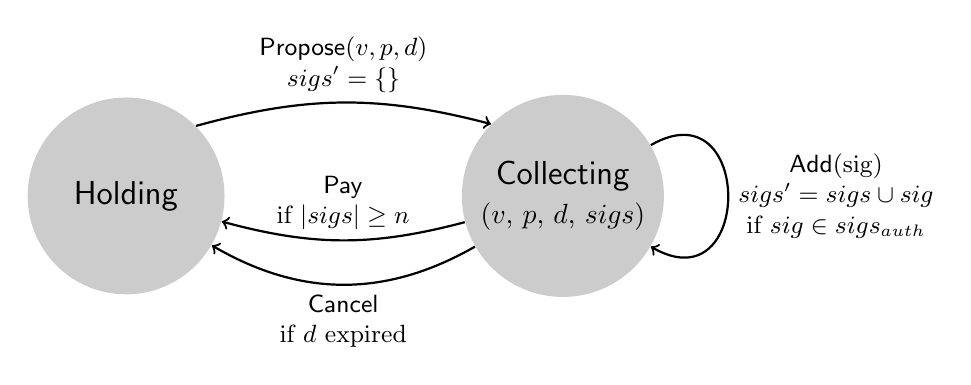
\begin{tikzpicture}[
    state/.style =
    { shape        = circle,
      fill         = gray!40,
      align        = center,
      font         = \large,
      minimum size = 2.5cm },
    transition/.style =
    { ->,
      thick },
    move/.style =
    { align  = center,
      anchor = center,
      font   = \small }
  ]
  \node[state] (a) {\Holding};
  \node[state, right = 3cm of a] (b) {\msf{Collecting}\\\normalsize ($v$, $p$, $d$, $sigs$)};

  \path
  (a.north east) edge[transition, bend left = 15]
    node[move, above] {$\Propose{v}{p}{d}$\\$sigs' = \{\}$}
  (b.north west)
  (b) edge[transition, out = 30, in = -30, looseness = 3]
      node[move, right] {\Add{sig}\\$sigs' = sigs \cup sig$\\ if $sig \in sigs_{auth}$}
      (b)
      edge[transition, bend left = 15]
      node[move, above] {\Pay\\if $|sigs| \geq n$}
      (a)
      edge[transition, bend left = 30]
      node[move, below] {\Cancel\\if $d$ expired}
      (a)
  ;
  \end{tikzpicture}
  \caption{Transition diagram for the multi-signature state machine;
    edges labelled with input from redeemer and transition constraints.}
  \label{fig:multisig-machine}
\end{figure}

A simple example for such a state machine is an on-chain $n$--of--$m$ multi-signature contract. Specifically, we have a given amount
$\val_\msc$ of some cryptocurrency and we require the approval of at
least $n$ out of an \textit{a priori} fixed set of $m \geq n$ owners to spend
$\val_\msc$. With plain \UTXO{} (e.g., on Bitcoin), a multi-signature
scheme requires out-of-band (off-chain) communication to collect all
$n$ signatures to spend $\val_\msc$. On Ethereum, and also in the
\EUTXO{} model, we can collect the signatures on-chain, without any
out-of-band communication. To do so, we use a state machine operating
according to the transition diagram in
Figure~\ref{fig:multisig-machine}, where we assume that the threshold
$n$ and authorised signatures $\sigs_\auth$ with \(|\sigs_\auth| = m\)
are baked into the contract code.

In the multi-signature state machine's implementation in the \EUTXO{} model, we use a validator
function $\nu_\msc$ accompanied by the datum $\delta_\msc$ to lock
$\val_\msc$. The datum $\delta_\msc$ stores the machine state,
which is of the form \(\Holding\) when only holding the locked value
or \(\Collecting{\val}{\kappa}{d}{\sigs}\) when collecting
signatures $\sigs$ for a payment of $\val$ to $\kappa$ by the deadline
$d$. The initial output for the contract is \((\nu_\msc, \val_\msc,
\Holding)\).

The validator $\nu_\msc$ implements the state transition diagram from
Figure~\ref{fig:multisig-machine} by using the redeemer of the spending input to determine the transition that needs to be taken. That redeemer (state machine input) can take four forms:
\begin{inparaenum}[(1)]
\item \(\Propose{\val}{\kappa}{d}\) to propose a payment of $\val$ to $\kappa$
  by the deadline $d$,
\item \(\Add{\sig}\) to add a signature $\sig$ to a payment,
\item $\Cancel$ to cancel a proposal after its deadline expired, and
\item $\Pay$ to make a payment once all required signatures have been collected.
\end{inparaenum}
It then validates that the spending transaction $\mi{tx}$ is a valid
representation of the newly reached machine state. This implies that
$\mi{tx}$ needs to keep $\val_\msc$ locked by $\nu_\msc$ and that the
state in the datum $\delta^{\prime}_\msc$ needs to be the successor state
of $\delta_\msc$ according to the transition diagram.

While the state machine in Figure~\ref{fig:multisig-machine} is fine, its mapping to \EUTXO\ transactions comes with a subtle caveat: what if, for a 2--of--3 contract, somebody posts a transition $\tx_{\mathrm{bad}}$ corresponding to the state \(\Collecting{\val}{\kappa}{d}{\{\sig_1, \sig_2\}}\) onto the chain \emph{without} going through any of the previous states, including without starting in $\Holding$?
Given that $\Pay$ merely checks \(|\sigs| \geq 2\), the payment would be processed when requested on $\tx_{\mathrm{bad}}$, even if \(\{\sig_1, \sig_2\}\) are invalid signatures.
We would not have been allowed to add the invalid signatures $\sig_1$ and $\sig_2$ by way of \(\Add{\sig}\) since its state transition checks signature validity, but by initialising the state machine in an intermediate state $s$ with \(\s{initial}(s) = \false\), we were able to circumvent that check.

In the plain \EUTXO\ model, there is no simple way for the validator implementing a state machine to assert that the state it is operating on arose out of a succession of predecessor states rooted in an initial state.
As a consequence of this limitation, the formal result presented in the \EUTXO\ paper~\cite{eutxo-1-paper} is not as strong as one might hope.
More precisely, this previous work did establish soundness and completeness for a weak bisimulation between CEMs and transactions on a \EUTXO\ ledger;
however, it fell short in that it did not show that an inductive property met by the states of a CEM may also be asserted for the corresponding states on the ledger.
The reason for this omission is precisely the problem we just discussed: for a ledger-representation of a CEM state, we can never be sure that it arose out of a transaction sequence rooted in an initial CEM state.

\subsection{Token provenance}
\label{sec:state-machine-provenance}

In the present work, we solve the problem described above. We will show that non-fungible tokens can be used to identify a unique trace of transactions through an \EUTXOma\ ledger that corresponds to all the states of the corresponding CEM. Moreover, we introduce a notion of \emph{token provenance} that enables us to identify the first CEM state in such a trace and to ensure that it is a state accepted by \(\s{initial} : \s{S} \rightarrow \B\). Together, these allow a state machine validator to ensure that a current CEM state indeed arose out of a trace of transactions rooted in a transaction corresponding to an initial CEM state merely by checking that the non-fungible token associated with this state machine instance is contained in the $\val$ of the state machine output that it locks: this would be $\val_\msc$ for the multi-signature contract of \S\ref{sec:cem-example}.

\section{Applications}
\label{sec:applications}

\UTXOma\ is able to support a large number of standard use cases for multi-asset ledgers, as well as some novel ones.
In this section we give a selection of examples.
There are some common themes: (1) Tokens as resources can be used to reify many non-obvious things, which makes them first-class tradeable items; (2) cheap tokens allow us to solve many small problems with \emph{more tokens}; and (3) the power of the scripting language affects what examples can be implemented.

\subsection{Simple single token issuance}
%
To create a simple currency $\mathsf{SimpleCoin}$ with a fixed supply of $\texttt{s = 1000 SimpleCoins}$ tokens, we might try to use the simple policy script $\texttt{Forges(s)}$ with a single forging transaction. Unfortunately, this is not sufficient as somebody else could submit another transaction forging another $\texttt{1000 SimpleCoins}$.

In other words, we need to ensure that there can only ever be a single transaction on the ledger that successfully forges $\mathsf{SimpleCoin}$. We can achieve that by requiring that the forging transaction consumes a specific \UTXO. As \UTXO{}s are guaranteed to be (1) unique and (2) only be spent once, we are being guaranteed that the forging policy can only be used once to forge tokens. We can use the script:

\begin{alltt}
  simple_policy(o, v) = SpendsOutput(o) && Forges(v)
\end{alltt}

\noindent where $\texttt{o}$ is an output that we create specifically for this purpose in a preceding setup transaction, and $\texttt{v = s}$.

\subsection{Reflections of off-ledger assets}
\label{sec:asset-tokens}

Many tokens are used to represent (be backed by) off-ledger assets on the ledger. An
important example of this is \emph{backed stablecoins}. Other noteworthy
examples of such assets include video game tokens, as well as service
tokens (which represent service provider obligations).

A typical design for such a system is that a trusted party (the ``issuer'') is responsible for creation and destruction of the asset tokens on the ledger.
The issuer is trusted to hold one of the backing off-ledger assets for every token that exists on the ledger, so the only role that the on-chain policy can play is to verify that the forging of the
token is signed by the trusted issuer.
This can be implemented with a forging policy that enforces
an $m$-out-of-$n$ multi-signature scheme, and no additional clauses:
\begin{alltt}
  trusted_issuer(msig) = JustMSig(msig)
\end{alltt}

\subsection{Vesting}

A common desire is to release a supply of some asset on some schedule.
Examples include vesting schemes for shares, and staged releases of newly minted tokens.
This seems tricky in our simple model: how is the forging policy supposed to know which tranches have already been released without some kind of global state which tracks them?
However, this is a problem that we can solve with more tokens. We start building
this policy by following the single issuer scheme, but we need to express more.

Given a specific output \code{o}, and two tranches of tokens \code{tr1} and \code{tr2} which should be released after \code{tick1} and \code{tick2}, we can write a forging policy such as:
\begin{alltt}
  vesting = SpendsOutput(o) && Forges(\cL"tr1" \mapsTo 1, "tr2" \mapsTo 1\cR)
         || TickAfter(tick1) && Forges(tr1bundle) && Burns(\cL"tr1" \mapsTo 1\cR)
         || TickAfter(tick2) && Forges(tr2bundle) && Burns(\cL"tr2" \mapsTo 1\cR)
\end{alltt}
%
This disjunction has three clauses:
\begin{itemize}
\item
  Once only, you may forge two unique tokens \code{tranche1} and \code{tranche2}.
\item
  If you spend and burn \code{tr1} and it is after \code{tick1}, then you may forge all the tokens in \code{tr1bundle}.
\item
  If you spend and burn \code{tr2} and it is after \code{tick2}, then you may forge all the tokens in \code{tr2bundle}.
\end{itemize}
%
By reifying the tranches as tokens, we ensure that they are unique and can be used precisely once.
As a bonus, the tranche tokens are themselves tradeable.

\subsection{Inventory tracker: tokens as state}

We can use tokens to carry some data for us, or to represent state.
A simple example is inventory tracking, where the inventory listing can only be modified by a set of trusted parties.
To track inventory on-chain, we want to have a single output containing all of the tokens of an ``inventory tracking'' asset.
If the trusted keys are represented by the multi-signature $\texttt{msig}$, the inventory tracker tokens should always be kept in a \UTXO\ entry with the following output:
\begin{alltt}
  (hash(msig) , \cL{}hash(msig) \mapsTo \cL{}hats \mapsTo 3, swords \mapsTo 1, owls \mapsTo 2\cR\cR)
\end{alltt}

The inventory tracker is
an example of an asset that should indefinitely be controlled by a specific script
(which ensures only authorized users can update the inventory), and
we enforce this condition in the forging script itself:

\begin{alltt}
  inventory_tracker(msig) = JustMSig(msig) && AssetToAddress(_)
\end{alltt}

In this case, $\texttt{inventory\_tracker(msig)}$ is both the forging
script and the output-locking script. The blank value supplied as the
argument means that the policy ID (and also the address) are both
assumed to be the hash of the $\texttt{inventory\_tracker(msig)}$
script.
Defined this way, our script is run at initial forge time, and any time
the inventory is updated. Each time
it only validates if all the inventory tracker tokens in the transaction's
outputs are always locked by this exact output script.

\subsection{Non-fungible tokens}

A common case is to want an asset group where \emph{all} the tokens are non-fungible.
A simple way to do this is to simply have a different asset policy for each token, each of which can only be run once by requiring a specific \UTXO\ to be spent. However, this is clumsy, and typically we want to have a set of non-fungible tokens all controlled by the same policy. We can do this with the \texttt{FreshTokens} clause.
If the policy always asserts that the token names are hashes of data unique to the transaction and token, then the tokens will always be distinct.

\subsection{Revocable permission}

An example where we employ this dual-purpose nature of scripts is revocable permission.
We will express permissions as a \emph{credential token}.

The list of users (as a list of hashes of their public keys) in a credential token is
composed by some central accreditation authority. Users usually trust that this authority
has verified some
real-life data, e.g. that a KYC accreditation authority has checked off-chain
that those it accredits meet some standard.\footnote{
KYC stands for ``know your customer'', which
is the process of verifying a customer's identity before allowing the customer
to use a company's service.
}
Note here that we significantly
simplify the function of KYC credentials for brevity of our example.

For example, suppose that
exchanges are only willing to transfer funds to those that have proved that
they are KYC-accredited.

In this case, the accreditation authority could issue an asset that looks like
\begin{alltt}
  \cL{}KYC_accr_authority \mapsTo \cL{}accr_key_1 \mapsTo 1, accr_key_2 \mapsTo 1, accr_key_3 \mapsTo 1\cR\cR
\end{alltt}

\noindent where the token names are the public keys of the accredited users.
We would like to make sure that

\begin{itemize}
  \item only the
authority has the power to ever forge or burn tokens controlled by this policy,
and it can do so at any time,
  \item all the users with listed keys are able to spend this asset
  as on-chain proof that they are KYC-accredited, and
  \item once a user is able to prove they have the credentials, they should be allowed
 to receive funds from an exchange.
\end{itemize}

We achieve this with a script of the following form:
\begin{alltt}
  credential_token(msig) = JustMSig(msig) && DoForge
                        || AssetToAddress(_) && Not DoForge && SignedByPIDToken(_)
\end{alltt}

Here, forges (i.e. updates to credential tokens) can only be done by the
$\texttt{msig}$ authority,
but every user whose key hash is included in the token names can spend from
this script, provided they return the asset to the same script.
To make a script that only allows spending from it if the user doing so
is on the list of key hashes in the credential token made by $\texttt{msig}$, we write

\begin{alltt}
  must_be_on_list(msig) = SpendsCur(credential_token(msig))
\end{alltt}

In our definition of the credential token, we have used all the strategies
we discussed above to extend the expressivity of an FPS language.
We are not yet using the \UTXO\ model to its full potential, as we are just
using the \UTXO\ to store some information that cannot be traded. However, we
could consider updating
our credential token use policy to associate spending it with another action,
such as adding a pay-per-use clause. Such a change really relies on the
\UTXO\ model.

\section{Meta-theoretical Properties of \EUTXOma}
\label{sec:formalization}

In~\cite{eutxo-1-paper}, we characterised the expressiveness of EUTXO
ledgers by showing that we can encode a class of state machines ---
\textit{Constraint Emitting Machines} (CEMs) --- into the ledger via a series
of transactions.  Formally, we showed that there is a weak
bisimulation between CEM transitions and their encoded
transitions in the ledger.

However, as we have seen from the example in \S\ref{sec:cem-example} above,
this result is not sufficient to allow us to reason about the properties
of the state machine.  Even if we know that each individual step is valid,
there may be some properties that are only guaranteed to hold if we started
from a proper initial state.
Specifically, we will not be able to establish any inductive or temporal property
unless we cover the base case corresponding to initial states.
Since our earlier model did not prevent
us from starting the ledger in an arbitrary (and perhaps non-valid) state, such
properties could not be carried over from the state machines to the
ledger.

In this section we extend our formalisation to map CEMs into threaded
ledgers.  By formalising some of the properties of \EUTXOma, we can
guarantee that a ledger was started from a valid initial state, and
thus carry over inductive and temporal properties from state machines.  All
the results in this section have been mechanised in Agda,
extending the formalisation from~\cite{eutxo-1-paper}.

\subsection{Token provenance}

Given a token in a \EUTXOma{} ledger, we can ask ``where did this token
\emph{come from}?''  Since tokens are always created in specific
forging operations, we can always trace them back through their
transaction graph to their \textit{origin}.

We call such a path through the transaction graph a \emph{trace}, and
define the \emph{provenance} of an asset at some particular output
to be a trace leading from the current transaction to an origin which
forges a value containing the traced tokens.

In the case of fungible tokens, there may be multiple possible traces:
since such tokens are interchangeable, if two tokens of some asset are forged separately, and then
later mingled in the same output, then we cannot say which one came from which forging.

Let $\nft = (p , a)$ denote a particular $\Asset\ a$ controlled by a $\Policy\ p$,
and $v^\nft = v(p)(a)$ the quantity of $\nft$ tokens present in value $v$.
$\Trace(l,o,\nft,n)$ is the type of sequences of transactions
$t_0,\dots, t_i, t_{i +1},\dots, t_k$ drawn from a ledger $l$ such that:
\begin{itemize}
\item the origin transaction $t_0$ forges at least $n$ $\nft$
  tokens: $t_0.\forge^\nft \ge n$
\item every pair $(t_i,t_{i + 1})$ has an input/output connection in
  the ledger that transfers at least $n$ $\nft$ tokens:
  $\exists o' \in t_{i + 1}.\inputs.\outputref. (t_i.\outputs[o'.\idx].\val^\nft \ge n)$
\item the last transaction $t_k$ carries the traced tokens in output $o$
\end{itemize}
We define $\Provenance(l,o,\nft)$ to be a
set of traces $\dots \Trace(l,o,\nft,n_i)\dots$, such that $\sum n_i \ge o.\val^\nft$.

To construct an output's provenance, with respect to
a particular policy and asset, we aggregate all possible
traces containing a token of this asset from the transaction's inputs as well
as from the value that is currently being forged.
Thus our tracing procedure will construct a sound over-approximation of the actual provenance.

\begin{displaymath}
\infer[\textsc{Provenance}]
  {\provenance(l,o,\nft) : \Provenance(l,o,\nft)}
  {o \in \{ t.\outputs \ | \ t \in l \}}
\end{displaymath}

\subsection{Forging policies are enforced}

One particular meta-theoretical property we want to check is
that each token is created properly: there is an origin transaction which forges
it and is checked against the currency's forging policy.

\begin{proposition}[Non-empty Provenance]
Given any token-carrying output of a valid ledger,
its computed provenance will be inhabited by at least one trace.

\begin{displaymath}
\infer[\textsc{Provenance}^+]
  {|\provenance(l, o, \nft)| > 0}
  {%
    o \in \{ t.\outputs \ | \ t \in l \}
  & o.\val^\nft > 0
  }
\end{displaymath}
\end{proposition}
%
However, this is not enough to establish what we want: due to
fungibility, we could identify a single origin as the provenance for
two tokens, even if the origin only forges a single token!

To remedy this, we complement (non-empty) token provenance with a
proof of \textit{global preservation}; a generalisation of the
local validity condition of \textit{value preservation} from
Rule~\ref{rule:value-is-preserved} in \S\ref{app:model}.

\begin{proposition}[Global Preservation]
Given a valid ledger $l$:
\begin{displaymath}
\sum_{t \in l} t.\forge = \sum_{o \in \unspent(l)} o.\val
\end{displaymath}
\end{proposition}

The combination of non-empty token provenance and global preservation
assures us that each token is created properly and there is globally
no more currency than is forged.

To prove these properties we require transactions to be unique
throughout the ledger, which is not implied by the validity rules of
Figure~\ref{fig:validity} in \S\ref{app:model}.  In practice though, one could derive
uniqueness from any ledger that does not have more than one
transaction with no inputs, since a transaction would always have to
consume some previously unspent output to pay its fees.
For our purposes, it suffices to assume there is always a single
\textit{genesis} transaction without any inputs:
\begin{displaymath}
\infer[\textsc{Genesis}]
  {|\{ t \in l\ | \ t.inputs = \emptyset \}| = 1}
  {}
\end{displaymath}
%
Then we can derive the uniqueness of transactions and unspent outputs.
%% \begin{minipage}{.45\linewidth}
%% \begin{displaymath}
%% \infer[\textsc{Unique-tx}]
%%   {\forall t_1, t_2 \in l.\ t_1 \neq t_2 }
%%   {\textsc{Genesis}}
%% \end{displaymath}
%% \end{minipage}
%% \begin{minipage}{.45\linewidth}
%% \begin{displaymath}
%% \infer[\textsc{Unique-utxo}]
%%   {\forall o_1, o_2 \in \unspent(l).\ o_1 \neq o_2 }
%%   {\textsc{Genesis}}
%% \end{displaymath}
%% \end{minipage}

\subsection{Provenance for non-fungible tokens}

However, our approach to threading crucially relies on the idea that a
non-fungible token can pick out a \emph{unique} path through the
transaction graph.

First, we define a token $\nft$ to be \textit{non-fungible} whenever
it has been forged at most once across all transactions of an existing
valid ledger $l$.
\ifootnote{%
  This really is a property of a particular ledger: a ``non-fungible'' token can become fungible in a longer ledger if other tokens of its asset are forged.
  Whether or not this is possible will depend on external reasoning about the forging policy.%
}
Then we can prove that non-fungible tokens have a singular provenance;
they really do pick out a unique trace through the transaction graph.

\begin{proposition}[Provenance for Non-fungible Tokens]
Given a valid ledger $l$ and an unspent output carrying a non-fungible
token $\nft$:

\begin{displaymath}
\infer[\textsc{NF-Provenance}]
  {|\provenance(l, o, \nft)| = 1}
  {%
    o \in \{ t.\outputs \ | \ t \in l \}
  & o.\val^\nft > 0
  & \sum_{t \in l} t.\forge^\nft \leq 1
  }
\end{displaymath}
\end{proposition}

\subsection{Threaded state machines}

Armed with the provenance mechanism just described, we are now ready
to extend the previously established bisimulation between CEMs and
state machines in ledgers, so that it relates CEMs with support for
initial states to \textit{threaded} state machines in ledgers.  That
is, in addition to creating an appropriate validator as
in~\cite{eutxo-1-paper}, we also create a forging policy that forges
a unique \textit{thread token} which is then required for the
machine to progress (and is destroyed when it terminates).  Crucially,
the forging policy also checks that the machine is starting in an
initial state.

For the sake of brevity, we refrain from repeating the entirety of
the CEM model definitions from~\cite{eutxo-1-paper}.
Instead, we focus only on the relevant modifications and refer
the reader to the mechanised model for more details.

First, we omit the notion of final states altogether, i.e., there is
no $\s{final}$ predicate in the definition of a CEM.
\ifootnote{%
  Note that this also simplifies the bisimulation propositions proven
  in~\cite{eutxo-1-paper}, since we no longer need to consider the
  special case of final states. Other than that, the statements stay
  exactly the same.%
}
We follow Robin Milner who observed, ``What matters about a sequence of
actions is not whether it drives the automaton into an accepting state
but whether the automaton is able to perform the sequence
interactively.''~\cite{milner-pibook} Formally, this corresponds to
prefix closure: if an automaton accepts a string $s$ then it accepts
any initial part of $s$~(Definition 2.6 \cite{milner-pibook}). Our
state machines are not classical state machines which accept or
reject a string --- rather they are \emph{interactive processes} which
respond to user input.
However, it might be useful to re-introduce final states in the future if we support burning of the thread token.

On the other hand, we now include the notion of initial state in the
predicate function $\initial : \s{S} \ra \B$, which characterises
the states in which a machine can start from. This enables us to ensure
that multiple copies of the machine with the same thread token cannot
run at once and the machine cannot be started in an intermediate state.
State machines whose execution must start from an initial state are also
referred to as \emph{rooted} state transition systems~\cite{TLSS}.

To enforce non-fungibility of the forged token, we require
that the forging transaction spends a specific output, fixed for a
particular CEM instance $\mathcal{C}$ and supplied along with its definition as a
field \s{origin}.  Therefore, since no output can be spent twice, we
guarantee that the token cannot be forged again in the future.

The CEM's forging policy checks that we only forge a single thread
token, spend the supplied origin, and that the state propagated in the
outputs is initial:

\begin{displaymath}
\polC(\mi{txInfo}, c) = \left\{
  \begin{array}{lll}
  \true  & \mi{if} \ \mi{txInfo}.\forge^\nft = 1 \\
         & \mi{and} \ \s{origin} \in \mi{txInfo}.\outputrefs \\
         & \mi{and} \ \initial(\mi{txInfo}.\mi{outputs}^\nft) \\
  \false & \mi{otherwise}
  \end{array}
\right.
\end{displaymath}
%
where $\nft = \{\hash{\valC} \mapsto \{ \hash{\polC} \mapsto 1 \}\}$
is the thread token and $\mi{txInfo}.outputs^\nft$ looks up the output
which carries the newly-forged thread token and is locked by the same
machine's validator, returning the datum decoded as a value of the
state type $\s{S}$.

We extend the previous definition of a CEM's validator (displayed in
grey) to also check that the thread token is attached to the source
state $s$ and propagated to the target state $s'$:

\begin{displaymath}
\color{gray}
\valC(s, i, \mi{txInfo}) = \left\{
  \begin{array}{ll}
  \true  & \mi{if}  \ \CStep{s} \\
         & \mi{and} \ \satisfies(\mi{txInfo}, \txeq) \\
         & \mi{and} \ \checkOutputs(s', \mi{txInfo}) \\
         & \begingroup\color{black}
           \mi{and} \ \s{propagates}(\mi{txInfo}, \nft, s, s')
           \endgroup \\
  \false & \mi{otherwise}
  \end{array}
\right.
\end{displaymath}

This is sufficient to let us prove a key result: given a threaded ledger
state (i.e., one that includes an appropriate thread token), that state
\emph{must} have evolved from a valid initial state.  Since we know
that the thread token must have a singular provenance, we know that
there is a unique ledger trace that begins by forging that token
--- which is guaranteed to be an initial CEM state.

\begin{proposition}[Initiality]
Given a valid ledger $l$ and an unspent output carrying the thread
token $\nft$, we can always trace it back to a single origin, which
forges the token and abides by the forging policy:
\end{proposition}
%
\begin{displaymath}
\infer[\textsc{Initiality}]
  { \exists tr. \ \s{provenance}(l, o, \nft) = \{ tr \}
  \ \land \
    \polC(\mkMpsContext(tr_0, \hash{\valC}, l^{tr_0})) = \true
  }
  {%
    o \in \{ t.\outputs \ | \ t \in l \}
  & o.\val^\nft > 0
  }
\end{displaymath}
%
where $tr_0$ denotes the origin of trace $tr$,
and $l^t$ is the prefix of the ledger up to transaction $t$.
The proof essentially relies on the fact that the thread token is
non-fungible, as its forging requires spending a unique output.
By \textsc{NF-Provenance}, we then get the unique trace back to a
\textit{valid} forging transaction, which is validated against the
machine's forging policy.

\subsection{Property preservation}

Establishing correct initialisation is the final piece we need to be
able to show that properties of abstract CEMs carry over to their
ledger equivalents.  It is no longer possible to reach any state that
cannot be reached in the abstract state machine, and so any properties
that hold over traces of the state machine also hold over traces of
the ledger.

Intuitively, looking at the ledger trace we immediately get from
\textsc{Initiality}, we can discern an underlying CEM trace
that throws away all irrelevant ledger information and only keeps
the corresponding CEM steps.
After having defined the proper notions of property preservation for
CEM traces, we will be able to transfer those for on-chain
traces by virtue of this extraction procedure.

A simple example of a property of a machine is an invariant. We
consider predicates on states of the machine that we call
state-predicates.
\begin{definition}
A state-predicate $P$ is an \emph{invariant} if it holds for all reachable
states of the machine. i.e., if it holds for the initial state, and
for any $s$, $i$, $s'$ and $\txeq$ such that $\CStep{s}$, if
it holds for $s$ then it holds for $s'$.
\end{definition}

\subsubsection{Traces of state machine execution.}
%
We have traced the path of a token through the ledger. We can also
trace the execution of a state machine. We consider rooted traces that
start in the initial state, and refer to them as just \emph{traces}. A
trace records the history of the states of the machine over time and
also the inputs that drive the machine from state to state.
\begin{definition}
A trace is an inductively defined relation on states:
\[
\infer[\mathsf{root}]
      {s \transTo s}
      {\initial(s) = \true}
\qquad
\infer[\mathsf{snoc}]
      {s \transTo s''}
      { s \transTo s'
      & \CStep{s'}
      }
\]
\end{definition}
%
This gives us a convenient notion to reason about temporal
properties of the machine, such as those which hold at all times, at
some time, and properties that hold until another one does. In this
paper we restrict our attention to properties that always hold.

\subsubsection{Properties of execution traces.}
%
Consider a predicate $P$ on a single step of execution.
A \textit{step-predicate} $P(s,i,s',\txeq)$ refers to the incoming state $s$, the input
$i$, the outgoing state $s'$ and the constraints $\txeq$. A
particularly important lifting of predicates on steps to predicates on
traces is the transformer that ensures the predicate holds for every
step in the trace.
\begin{definition}
Given a step-predicate $P$, a trace $tr$ satisfies $\All(P,tr)$
whenever every step $\CStep{s}$ satisfies $P(s,i,s',\txeq)$.
\end{definition}
A predicate transformer lifting state-predicates to a predicate that
holds everywhere in a trace can be defined as a special case:
$\AllS(P,tr) = \All(\lambda s\ i\ s'\ \txeq.\ P(s) \land P(s'),\ tr)$.

We are not just interested in properties of CEM traces in
isolation, but more crucially in whether these
properties hold when a state machine is compiled to a contract to be
executed on-chain.

We observe that the on-chain execution traces precisely follow the
progress of the thread token. We use the same notion of token
provenance to characterise on-chain execution traces. To facilitate
reasoning about these traces, we can \emph{extract} the corresponding
state machine execution traces and reason about those. This allows us
to confine our reasoning to the simpler setting of state machines.

\begin{proposition}[Extraction]
\label{prop:extraction}
Given a valid ledger $l$ and a singular provenance of the
\textup{(}non-fungible\textup{)} thread token $\nft$, we can extract a rooted state
machine trace.
\end{proposition}

\begin{displaymath}
\infer[\textsc{Extraction}]
  {tr.source \transTo tr.destination}
  {\provenance(l, o, \nft) = \{ tr \}}
\end{displaymath}
where $tr.source, tr.destination$ are the states associated with the endpoints of the trace $tr$.
\begin{proof}
  It is straightforward to show this holds, as a corollary of
  \textsc{Initiality}. For the base case, knowing that the origin of the
  trace abides by the forging policy ensures that it forges the thread
  token and outputs an initial state (\s{root}). In the inductive
  step, knowing that the validator runs successfully guarantees that
  there is a corresponding CEM step (\s{snoc}).
  \qed
\end{proof}

\begin{corollary}
\label{all-cor}
Any predicate that always holds for a CEM trace also holds for the one
extracted from the on-chain trace.
\end{corollary}
%
We will write $\extract(tr)$ whenever we want to extract the CEM trace from the on-chain trace $tr$.

\begin{example}
Consider a CEM representing a simple counter that counts up from
zero:
\[
\begin{array}{l}
  (\mathbb {Z}, \{\mathsf{inc}\}, \step, \initial)\quad
  \mathbf{where}\quad
  \step(i,\mathsf{inc}) = \mathsf{just}(i + 1);\quad
  \initial(0) = \true\\
\end{array}
\]
\end{example}
%
A simple property that we want to hold is that the state of the
counter is never negative.

\begin{property}
\label{prop:non-negative}
The counter state $c$ is non-negative, i.e., $c \geq 0$.
\end{property}

\begin{lemma}
\label{counter-inv}
Property~\ref{prop:non-negative} is an invariant, i.e., it holds for all reachable states:
  \begin{enumerate}
  \item $\forall c.\ \initial(c) \rightarrow c \geq 0$
  \item $\forall c\ c'.\ \CStep{c} \rightarrow c\geq 0 \rightarrow c' \geq 0$
  \end{enumerate}
\end{lemma}

\begin{proposition}
In all reachable states, both off-chain and on-chain, the counter is non-negative.
\end{proposition}
\begin{enumerate}
\item $\forall c\ c'\ (tr : c \transTo c').\ \AllS(\lambda x.\ x \geq 0,\ tr)$
\item $\forall l\ o\ tr.\ {\provenance(l, o, \nft) = \{ tr \}} \rightarrow \AllS(\lambda x.\ x \geq 0, \extract(tr))$
\end{enumerate}
\begin{proof}
  (1) follows from Lemma~\ref{counter-inv}. (2) follows from (1) and Corollary~\ref{all-cor}.
  \qed
\end{proof}

\begin{example}
We return to the $n$--of--$m$ multi-signature contract of
\S\ref{sec:EUTXOma}. We pass as parameters to the machine a
threshold number $n$ of signatures required and a list of $m$ owner
public keys \textit{signatories}. The states of the machine are given by
$\{\Holding, \msf{Collecting}\}$ and the
inputs are given by $\{\Pay, \Cancel, \msf{Add}, \msf{Propose}\}$,
along with their respective arguments.
The only initial state is $\Holding$ and we omit the definition of
$\step$ which can be read off from the picture in
Figure~\ref{fig:multisig-machine}.

First and foremost, the previous limitation of starting in non-initial
states has now been overcome, as proven for all state machines in
Proposition~\ref{prop:extraction}.
Specifically, this holds at any output in the ledger carrying the
$\msf{Collecting}$ state,
therefore it is no longer possible to circumvent the checks performed
by the $\msf{Add}$ input.

\end{example}
\begin{property}
It is only possible to cancel after the deadline.
\end{property}
%
We define a suitable step predicate $Q$ on inputs and constraints for a step. If the input is
$\Cancel$ then the constraints must determine that the
transaction can appear on the chain only after the deadline. If the
input is not $\Cancel$ then the predicate is trivially
satisfied.
\begin{displaymath}
Q(s,i,\_,\txeq) = \left\{
  \begin{array}{ll}
  \false & \mi{if}  \ i = \Cancel \ \mi{and}\ s = \Propose{\_\ }{\_\ }{d} \ \mi{and}\ \txeq.\s{range} \neq d\dots\!+\!\infty \\
  \true  & \mi{otherwise}
  \end{array}
\right.
\end{displaymath}
%
Note that we could extend $Q$ to include cases for correctness
properties of other inputs such as ensuring that only valid signatures
are added and that payments are sent to the correct recipient.
\begin{lemma}
\label{lem:msig-correct}
$Q$ holds everywhere in any trace. i.e. $\forall s\ s'\ (tr : s \transTo s').\ \All(Q,\ tr)$.
\end{lemma}
\begin{proof}
  By induction on the trace $tr$.
  \qed
\end{proof}
\begin{proposition}
  For any trace, all cancellations occur after the deadline.
\end{proposition}
\begin{proof}
  Follows from Lemma~\ref{lem:msig-correct} and the fact that the validator ensures all constraints are satisfied.
  \qed
\end{proof}

\paragraph{Beyond safety properties.}
All the properties presented here are \textit{safety} properties, i.e., they hold in every state and we express them as state predicates.
However, a large class of properties we would like to prove are \textit{temporal}, as in relating different states (also known as \textit{liveness} or \textit{progress} properties~\cite{manna-pnueli,baier-katoen}).

Scilla, for instance, provides the \texttt{since\_as\_long} temporal operator for such purposes~\cite{scilla},
which we have also encoded in our framework using a straightforward inductive definition.
However, one may need to move to infinitary semantics to encode the entirety of \textit{Linear Temporal Logic} (LTL)
or \textit{Computational Tree Logic} (CTL), in contrast to reasoning only about finite traces.
In our setting, we would need to provide a \textit{coinductive} definition of traces
to encode the temporal operators of the aforementioned logics,
as done in \cite{infinite-trees} in the constructive setting of the Coq proof assistant.
We leave this exploration for future work.

\section{Related work}
\label{sec:related-work}

We discuss other efforts to use state machines to model smart
contracts in our previous paper~\cite{eutxo-1-paper} and we compare our
 approach to a multi-asset ledger with other systems (including Waves~\cite{waves}, Stellar~\cite{stellar}, and Zilliqa~\cite{scilla-arxiv}) in the companion
paper~\cite{plain-multicurrency}.
Here we focus on approaches that reason formally about the
properties of such contracts as state machines, which is the essence
of this paper's main contribution.
We do not know of any other approaches that use tokens as state threads.

\paragraph{Scilla.}
%
Scilla~\cite{scilla} is a intermediate-level language for writing smart
contracts as state machines.
The Scilla authors have used Coq to reason about contracts written in
Scilla, proving a variety of temporal properties such as safety,
liveness, and others; hence their goals are similar to ours.
Since our meta-theory enjoys property preservation over any trace predicate,
we can also formally prove these temporal properties.

However, we are targeting a very different ledger model.
This means that we need to do additional work: the major contribution
of this paper is using tokens to provide state machine instances with
an ``identity'', which comes for free on Ethereum.
Another Ethereum feature that widens the gap between our approaches is
support for asynchronous message passing,
which renders Scilla unsuitable as a source language for a
\UTXO{}-based ledger,
and explains the different choice of \textit{communicating automata}~\cite{scilla-arxiv}
as the backbone of its model.
Nonetheless, it would be interesting to develop a Scilla-like language
that was suitable for our ledger model.

\paragraph{BitML.}
%
The \textit{Bitcoin Modelling Language} (BitML)~\cite{bitml} allows the definition
of smart contracts running on Bitcoin by means of a restricted class
of state machines.
The BitML compilation process has been proven to be computationally
sound (although this proof has not yet been mechanised), which allows
trace-based properties about the BitML contract to be transferred to
the implementation, as in our system.
This proof is used, for example, in~\cite{atzei2019developing} to prove
and transfer LTL properties of BitML contracts to their implementations.
Most importantly, LTL formulas can be automatically verified using a dedicated \textit{model checker}.

Again, our work is closely related in spirit, although our ledger
model is different and we use a more expressive class of state
machines. In the future, we plan to add support for LTL formulas in our framework.

\paragraph{VeriSolid.}
%
VeriSolid~\cite{mavridou2019verisolid} synthesises Solidity smart
contracts from a state machine specification, and verifies temporal
properties of the state machine using CTL.
They use this to prove safety, liveness, deadlock-freedom, and others.
Again, we expect to support CTL formulas in the near future.

In contrast, the present work focuses on establishing a formal
connection between the state machine model and the real implementation
on the ledger --- in particular, our proofs are mechanised.
We also target a \UTXO\ ledger model, whereas VeriSolid targets the Ethereum ledger.
Finally, our approach is agnostic about the logic or checker used to
prove the properties that we assert on state machines and, by way of
the results in this paper, transfer to an \EUTXOma\ implementation of
the same state machine.

\subsubsection*{Acknowledgments.} We thank Gabriele Keller for comments on an earlier version of this paper.


\bibliographystyle{splncs04}
\bibliography{eutxoma}

\appendix
\newpage
\section{Complete formal definition of \EUTXOma}
\label{app:model}

\subsection{Finitely-supported functions.}
\label{sec:fsfs}

If $K$ is any type and $M$ is a monoid with identity element $0$, then a function $f: K \rightarrow M$ is \textit{finitely supported} if $f(k) \ne 0$ for only finitely many $k \in K$.
More precisely, for $f: K \rightarrow M$ we define the \textit{support} of $f$ to be
%%
$\supp(f) = \{k \in K : f(k) \ne 0\}$
%%
and
%%
$\FinSup{K}{M} = \{f : K \rightarrow M : \left|\supp(f)\right| < \infty \}$.
%%

If $(M,+,0)$ is a monoid then $\FinSup{K}{M}$ also becomes a monoid if we define addition pointwise ($(f+g)(k) = f(k) + g(k)$), with the identity element being the zero map.
Furthermore, if $M$ is an abelian group then $\FinSup{K}{M}$ is also an abelian group under this construction, with $(-f)(k) = -f(k)$.
Similarly, if $M$ is partially ordered, then so is $\FinSup{K}{M}$ with comparison defined pointwise: $f \leq g$ if and only if $f(k) \leq g(k)$ for all $k \in K$.

It follows that if $M$ is a (partially ordered) monoid or abelian group then so is $\FinSup{K}{\FinSup{L}{M}}$ for any two sets of keys $K$ and $L$.
We will make use of this fact in the validation rules presented later (see Figure~\ref{fig:validity}).

Finitely-supported functions are easily implemented as finite maps, with a failed map lookup corresponding to returning 0.

\subsection{Ledger types}

The formal definition of the \EUTXOma\ model integrates token bundles and forge fields from the plain \UTXOma\ model~\cite{plain-multicurrency} into the single currency \EUTXO\ model definition, while adapting forging policy scripts to enjoy the full expressiveness of validators in \EUTXO\ (rather than the limited domain-specific language of \UTXOma). Figures~\ref{fig:eutxo-types} and~\ref{fig:ctx-types} define the ledger types for \EUTXOma.
%
%
\begin{ruledfigure}{t}
  \begin{displaymath}
    \begin{array}{rll}
      \multicolumn{3}{l}{\textsc{Basic types}}\\
     \B, \N, \Z && \mbox{the type of Booleans, natural numbers, and integers}\\
      \H{} && \mbox{the type of bytestrings: } \bigcup_{n=0}^{\infty}\{0,1\}^{8n}\\g
      (\phi_1 : T_1, \ldots, \phi_n : T_n) && \mbox{a record type with fields $\phi_1, \ldots, \phi_n$ of types $T_1, \ldots, T_n$}\\
      t.\phi && \mbox{the value of $\phi$ for $t$, where $t$ has type $T$ and $\phi$ is a field of $T$}\\
      \Set{T} && \mbox{the type of (finite) sets over $T$}\\
      \List{T} && \mbox{the type of lists over $T$, with $\_[\_]$ as indexing and $|\_|$ as length}\\
      h::t && \mbox{the list with head $h$ and tail $t$}\\
%      x \mapsto f(x) && \mbox{an anonymous function}\\
%      \hash{c} && \mbox{a cryptographic collision-resistant hash of $c$}\\
      \Interval{A} && \mbox{the type of intervals over a totally-ordered set $A$}\\
      \FinSup{K}{M} && \mbox{the type of finitely supported functions from a type $K$ to a monoid $M$}\\
      \\
      \multicolumn{3}{l}{\textsc{Ledger primitives}}\\
      \Quantity && \mbox{an amount of an assets}\\
      \Asset && \mbox{a type consisting of identifiers for individual asset classes}\\
      \Tick && \mbox{a tick}\\
      \Address && \mbox{an ``address'' in the blockchain}\\
      \Data && \mbox{a type of structured data}\\
      \DataHash && \mbox{the hash of a value of type \Data{}}\\
      \hashData : \Data \rightarrow \DataHash && \mbox{computes the hash of an value of type\Data}\\
      \TxId && \mbox{the identifier of a transaction}\\
      \txId : \eutxotx \rightarrow \TxId && \mbox{computes the identifier of a transaction}\\
      \lookupTx : \Ledger \times \TxId \rightarrow \eutxotx{} && \mbox{retrieves the unique transaction with a given identifier}\\
      \Script && \mbox{the (opaque) type of scripts}\\
      \applyScript{\_}: \Script \rightarrow \Data \times \cdots \times \Data \rightarrow \B && \mbox{applies a script to its arguments}\\
      \scriptAddr : \Script \rightarrow \Address && \mbox{the address of a script}\\
\\
    \multicolumn{3}{l}{\textsc{Defined types}}\\
    \Policy  &=& \Address\\
    \Signature &=& \H\\
    \\
    \Quantities   &=& \FinSup{\Policy}{\FinSup{\Asset}{\Quantity}}\\
    \\
    \Output &=&(\addr: \Address, \val: \Quantities, \datumHash: \DataHash)\\
    \\
    \OutputRef &= &(\txrefid: \TxId, \idx: \s{Int})\\
    \\
    \Input &=&( \outputref: \sf{OutputRef},\\
                & &\ \validator: \Script,\\
                & &\ \datum: \Data,\\
                & &\ \redeemer: \Data)\\
    \\
    \eutxotx &=&(\inputs: \Set{\Input},\\
               & &\ \outputs: \List{\Output},\\
               & &\ \i{validityInterval}: \Interval{\Tick},\\
               & &\ \forge: \Quantities,\\
               & &\ \forgeScripts: \Set{\Script},\\
               & &\ \sigs: \Set{\Signature})\\
    \\
    \Ledger &=&\!\List{\eutxotx}\\
    \end{array}
  \end{displaymath}
  \caption{Primitives and basic types for the \EUTXOma{} model}
  \label{fig:eutxo-types}
\end{ruledfigure}
%
\begin{ruledfigure}{t}
  \begin{displaymath}
  \begin{array}{rll}
    \s{OutputInfo}\s{ } &=&(\val: \Quantities,\\
                          & &\ \i{validatorHash}: \Address,\\
                          & &\ \datumHash: \DataHash)\\
    \\
    \s{InputInfo}\s{ } &=& (\outputref: \s{OutputRef},\\
                         & &\ \i{validatorHash}: \Address,\\
                         & &\ \i{datumHash}: \DataHash,\\
                         & &\ \i{redeemerHash}: \DataHash,\\
                         & &\ \val: \Quantities)\\
     \\
     \s{TxInfo}\s{ } &=&(\i{inputInfo}: \List{\s{InputInfo}},\\
                 & &\ \i{outputInfo}: \List{\s{OutputInfo}},\\
                 & &\ \i{validityInterval}: \Interval{\Tick},\\
                 & &\ \forge: \Quantities,\\
                 & &\ \forgeScripts: \Set{\Script},\\
                 & &\ \sigs: \FinSet{\Signature})\\
    \\
    \s{\vlctx}\s{ } &=& (\s{TxInfo}, \N) \\
    \s{\mpsctx}\s{ } &=& (\s{TxInfo}, \Policy) \\
    \\
    \mkVlContext: \eutxotx \times \s{Input} \times \Ledger & \rightarrow &\vlctx\\
                     & &   \mbox{\parbox[t]{55mm}{summarises a transaction for a validator script in the context of an input and a ledger state}}\\
 \\
    \mkMpsContext: \eutxotx \times \Policy \times \Ledger & \rightarrow & \mpsctx\\
                     & &   \mbox{\parbox[t]{55mm}{summarises a transaction for a forging policy script in the context of an currency and a ledger state}}\\
  \end{array}
  \end{displaymath}
  \caption{The \ctx{} types for the \EUTXOma{} model}
  \label{fig:ctx-types}
\end{ruledfigure}

\subsection{Transaction validity}

\begin{ruledfigure}{t}
  \begin{displaymath}
    \begin{array}{lll}
      \multicolumn{3}{l}{\txunspent : \eutxotx \rightarrow \Set{\s{OutputRef}}} \\
      \txunspent(t) &=& \{(\txId(t),1), \ldots, (\txId(id),\left|t.outputs\right|)\}\\
      \\
      \multicolumn{3}{l}{\unspent : \s{Ledger} \rightarrow \Set{\s{OutputRef}}} \\
      \unspent([]) &=& \emptymap \\
      \unspent(t::l) &=& (\unspent(l) \setminus t.\inputs) \cup \txunspent(t)\\
      \\
      \multicolumn{3}{l}{\getSpent : \s{Input} \times \s{Ledger} \rightarrow \s{Output}}\\
      \getSpent(i,l) &=& \lookupTx(l, i.\outputref.\id).\outputs[i.\outputref.\idx]
    \end{array}
  \end{displaymath}
  \caption{Auxiliary functions for \EUTXOma{} validation}
  \label{fig:validation-functions}
\end{ruledfigure}
%
\begin{ruledfigure}{t}
\begin{enumerate}

\item
  \label{rule:slot-in-range}
  \textbf{The current tick is within the validity interval}
  \begin{displaymath}
    \msf{currentTick} \in t.\i{validityInterval}
  \end{displaymath}

\item
  \label{rule:all-outputs-are-non-negative}
  \textbf{All outputs have non-negative values}
  \begin{displaymath}
    \textrm{For all } o \in t.\outputs,\ o.\val \geq 0
  \end{displaymath}

\item
  \label{rule:all-inputs-refer-to-unspent-outputs}
  \textbf{All inputs refer to unspent outputs}
  \begin{displaymath}
    \{i.\outputref | i \in t.\inputs \} \subseteq \unspent(l).
  \end{displaymath}

\item
  \label{rule:value-is-preserved}
  \textbf{Value is preserved}
  \begin{displaymath}
    t.\forge + \sum_{i \in t.\inputs} \getSpent(i, l) = \sum_{o \in t.\outputs} o.\val
  \end{displaymath}

\item
  \label{rule:no-double-spending}
  \textbf{No output is double spent}
  \begin{displaymath}
    \textrm{If } i_1, i \in t.\inputs \textrm{ and }  i_1.\outputref = i.\outputref
    \textrm{ then } i_1 = i.
  \end{displaymath}

\item
  \label{rule:all-inputs-validate}
  \textbf{All inputs validate}
  \begin{displaymath}
    \textrm{For all } i \in t.\inputs,\ \applyScript{i.\validator}(i.\datum,\, i.\redeemer,\, \toData(\mkVlContext(t, i, l))) = \true
  \end{displaymath}

\item
  \label{rule:validator-scripts-hash}
  \textbf{Validator scripts match output addresses}
  \begin{displaymath}
    \textrm{For all } i \in t.\inputs,\ \scriptAddr(i.\validator) = \getSpent(i, l).\addr
  \end{displaymath}

\item
  \label{rule:datum-objects-hash}
  \textbf{Datum objects match output hashes}
  \begin{displaymath}
    \textrm{For all } i \in t.\inputs,\ \hashData(i.\datum) = \getSpent(i, l).\datumHash
  \end{displaymath}

\item
  \label{rule:forging}
  \textbf{Forging}\\
  A transaction with a non-zero \forge{} field is only
  valid if either:
  \begin{enumerate}
  \item the ledger $l$ is empty (that is, if the transaction is the initial transaction).
  \item \label{rule:custom-forge}
    for every key $h \in \supp(t.\forge)$, there
    exists $s \in t.\forgeScripts$ with
    $\scriptAddr(s) = h$.
  \end{enumerate}
\medskip % items jammed together without this
\item
  \label{rule:all-mpss-run}
  \textbf{All forging policy scripts validate}
  \begin{displaymath}
    \textrm{For all } s \in t.\forgeScripts,\ \applyMPScript{s}(\toData(\mkMpsContext(t, \scriptAddr(s), l))) = \true
  \end{displaymath}

\end{enumerate}
\caption{Validity of a transaction $t$ in the \EUTXOma{} model}
\label{fig:validity}
\end{ruledfigure}
%
Finally, we provide the transaction validity rules, which among other things state how forging policy scripts affect transaction validity. To this end, we replace the notion of an integral $\Quantity$ for values by the token bundles discussed in \S\ref{sec:informal-token-bundles} and represented by values of the type $\Quantities$.

As indicated in \S\ref{sec:informal-eutxo}, validator scripts get a context argument, which includes the validated transaction as well as the outputs that it consumed, in \EUTXO. For \EUTXOma, we need two different such context types. We have $\vlctx$ for validators and $\mpsctx$ for forging policies. The difference is that in $\vlctx$ we indicate the input of the validated transaction that consumes the output locked by the executed validator, whereas for forging policies, we provide the policy script hash. The latter makes it easy for the policy script to look up the component of the transaction's forging field that it is controlling.

The validity rules in Figure~\ref{fig:validity} define what it means for a transaction $t$ to be valid for a valid ledger $l$ during the tick \currentTick. (They make use of the auxiliary functions in Figure~\ref{fig:validation-functions}.) Of these rules, Rules~\ref{rule:slot-in-range},~\ref{rule:all-outputs-are-non-negative},~\ref{rule:all-inputs-refer-to-unspent-outputs},~\ref{rule:value-is-preserved}, and~\ref{rule:no-double-spending} are common to the two systems (\EUTXO\ and \UTXOma) that we are combing here; Rules~\ref{rule:all-inputs-validate} and~\ref{rule:validator-scripts-hash} are similar in both systems, but we go with the more expressive ones from \EUTXO. The crucial changes are to the construction and passing of the context types mentioned above, which appear in Rules~\ref{rule:all-inputs-validate} and~\ref{rule:all-mpss-run}. The later is the main point as it is responsible for execution of forging policy scripts.

A ledger $l$ is \textit{valid} if either $l$ is empty or $l$ is of the form $t::l^{\prime}$ with $l^{\prime}$ valid and $t$ valid for $l^{\prime}$.


\end{document}
